\documentclass[midd]{thesis}

\usepackage{graphicx}
\usepackage{times}
\usepackage{amsmath}
\usepackage{booktabs}
\usepackage{lscape}
\usepackage[table,xcdraw]{xcolor}

\bibliographystyle{plain}
\title {Computational Aesthetic Evaluation using Convolutional Neural Networks}
\author {Teddy Knox}
\adviser {Professor Christopher Andrews}

\begin{document}
\maketitle









\begin{abstract}
The accuracies of state-of-the-art machine learning techniques have exceeded the accuracy of humans at certain limited tasks, suggesting the computers will soon be able to complete many sophisticated tasks competently. This study tested the accuracy of state-of-the-art convolutional neural networks for modeling the statistically-defined visual aesthetic tastes of randomly generated triangle art. Our trained model demonstrated no predictive power at this task. Further research will be needed to interpret this result.
\end{abstract}

\begin{acknowledgements}
I dedicate this paper to science.
\end{acknowledgements}

\contentspage
\tablelistpage
\figurelistpage

\normalspacing \setcounter{page}{1} \pagenumbering{arabic}
















\chapter{Introduction}
\label{sec:intro}

% TODO: Cite better than human performance from machine learning

% general introduction to CAE and generative art
% why we would care? vision
% WHat is this particular thesis about -> applying ml to the problem
% what are we doing? -> convolutional neural network
% more specific -> ran a study, using GoogLeNet
% What we will discuss ->

Machine learning is a broad discipline of computer science that has seen rapid advances in recent years, and has the potential to impact all human enterprises. The latest algorithms are capable of competitive or even better-than-human performance [citation needed] on certain tasks, and their applications are increasing in proportion to the availability of training data. One such application will be in the field of generative art and design. Generative art is art that is created procedurally, often with the help of a computer. Until recently, the use of computers in art and design has been limited to rote tasks such as preparing renderings and generating randomness, but advances in machine learning may soon enable computers to contribute higher-level aspects of the creative process, such as creative generation and aesthetic evaluation. Computation Aesthetic Evaluation (CAE) is the problem in generative art research of programming a computer to subjectively differentiate between aesthetically pleasing and displeasing content. This problem is important to the field of generative art for its potential to automate searches for aesthetic solutions, and would also be useful for building personalized recommendation systems. This research investigates the applicability of state-of-the-art general-purpose pattern recognition algorithms to computational aesthetic evaluation. This experimentation is motivated by an interest in discovering the limits of these impressive models. By evaluating their accuracy on unconventional datasets of unknown complexity, we hope to gain a better understanding of both the model's capabilities and the hidden structure of the dataset. This paper first provides background and formulates the problem, then explains the experimentation in detail, and concludes with a discussion of results and future uses of machine learning models for the analysis of artistic content.

% TODO: Position xkcd graphic connoisseur.png https://xkcd.com/915/
\begin{figure}
\centering
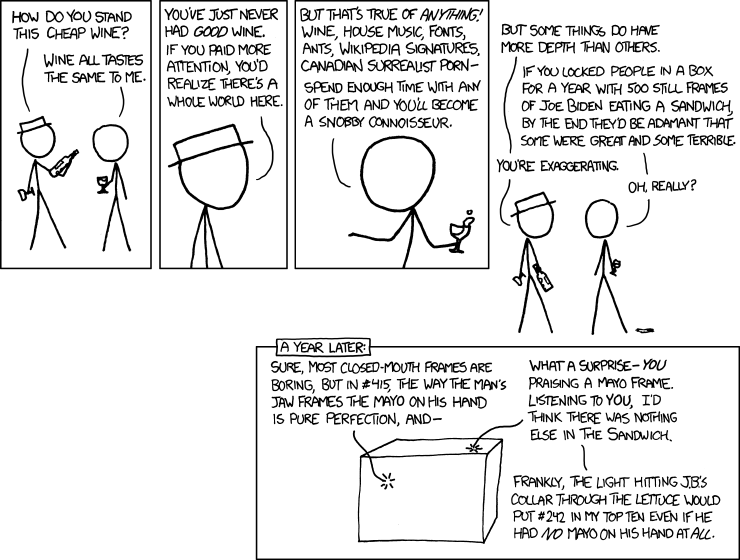
\includegraphics[width=0.9\textwidth]{visualizations/connoisseur.png}
\caption{Relevant xkcd: Aesthetic judgements can be arbitrarily esoteric.}
\label{fig:effectivecomplexity}
\end{figure}

Convolutional Neural Networks (CNNs) are a type of model inspired by the biology of the human visual processing center, and have been shown to be the most effective model for image recognition to date.
% TODO: Cite this assertion
CNNs are a type of feed-forward artificial neural network architecture formed by layers of convolutional filters, trained to derive high-level features from low-level pixel data. These high-level features are powerful and versatitle data separators which are then typically fed into a non-linear classifier or regressor to produce final predictions. The network's parameters are learned through an iterative training process, where batches of examples are fed into the network and network parameters are adjusted to reduce prediction errors. Iterations of adjustments are made until the network's prediction accuracy on its training data converges or surpasses a threshold.
























\chapter{Background}
Before examining this study we will explain background principles in the fields of Computational Aesthetics and Image Recognition.

\section{Computational Aesthetics}
Computational aesthetics is a fledgeling interdisciplinary field formed by the overlap of research in machine learning, neuroethetics, and evolutionary psychology. Efforts in this field are mostly explorational, and few concrete advances have been made. Some of the most-cited papers in the field of Computational Aesthetics are titled ``Computational aesthetic evaluation: Past and future'', ``Defining computational aesthetics'', and ``Experiments in computational aesthetics'', which intuitively indicate the field's stage of advances. These studies fall into practical and theoretical categories, roughly corresponding to top-down and bottom-up research strategies. Practical studies are oriented around conducting experiments to verify the correlation of commonly-held art school heuristics with subjective aesthetic ratings, in an effort make generalizations. Theoretical studies aim to develop a connectionist model for understanding aesthetics by drawing upon the insights of machine learning and neuroaethetics \cite{galanter2012computational, hoenig2005defining, machado2008experiments}.

% TODO: Talk about top-down work

The bottom-up work in computational aesthetics aims to develop an enlightened philosophical framework for understanding the human aesthetic system, and is indispensible for thinking clearly about bottom-up experimental work. Galanter and Hoenig grapple head-on with the field's conceptual entanglement, with an awareness of the ``baby steps'' that any progress will look like. We suspect, and we think these researchers would agree, that generalizable advances in this field will be deeply related to machine learning and neuroesthetics (the biological study of aesthetics), rather than more practical areas of aesthetics offering guidelines like the Gestalt laws. Given that philosophers have been devising high-level heuristics for judging aesthetics since antiquity, it seems unlikely that the increased availability of computational power will directly impact our conception of the problem.

To provide context, we will briefly summarize the history of computational aesthetics, and then categorize and summarize recent research strategies.

\subsection{Philosophical Underpinnings Computational Aesthetics}

One of the first significant advances in the greater philosophy of aesthetics is owed to Mathematician G.D. Birkoff, who spent a year traveling the world to study beauty across cultures, before proposing a speculative psychological model for quantifying it. In his oft-referenced 1933 paper \emph{Aesthetic Measure}, Birkoff proposes that the perception of beauty is the pleasurable resolution of apparent complexity of a stimulus into a compact mental representation. He codified this relationship into a formula that relates degree of beauty $B$ to the balanced ratio of order $O$ to complexity $C$.

\begin{align*}
B &= \frac{O}{C}
\end{align*}

The plausibility of Birkoff's measure as a guiding philosophy of aesthetics earned it significant attention in later experimental studies. The recent work of Ragau et. al. and Koshel et. al. draws from information theory to approximate the parameters of Birkoff's formula. They used zeroth-order measures such as Kolmogorov complexity and Shannon entropy \cite{rigau-1, koshelev-1}, to demonstrate encouraging correlations between Birkoff's measure and human-rated beauty.

These results are significant enough to validate the direction Birkoff's core idea --- that the human aesthetic response is tuned to respond to stimuli that are sophisticated yet digestible. Novel ideas in the fields of machine learning, neuroesthetics, and the emerging field of evolutionary philosophy (The top-down study of evolutionary adaptations), may be a way forward.
% TODO: rework the following
Philip Galanter stands at the intersection of these fields, and subscribes to the view that humans find stimuli with the greatest ``effective complexity'' to be the most engaging, and thus the most rewarding. Within this framework, the problem of computational aesthetics can be expressed as the study of how humans judge ``effective complexity'' \cite{galanter-1,galanter-2,galanter-3,galanter-4}. Effective complexity is a theoretical measure conceived by Gell-Man et. al. \cite{gell2004effective} to roughly correspond to the colloquial meaning of the word ``complex''. Effective complexity measures resistance to entropic forces rather than resistance to signal compression. For example, a symphony by Mozart possesses greater effective complexity than white noise, because it presents a manageable amount of harmonious sophistication for us to process.

\begin{figure}
\centering
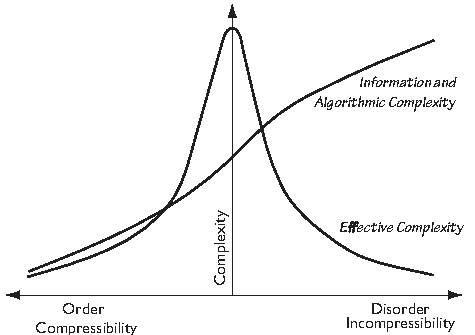
\includegraphics[width=0.75\textwidth]{figures/effectivecomplexity.pdf}
\caption{Relationship between effective complexity and order}
\label{fig:effectivecomplexity}
\end{figure}

In seeking to develop a computational aesthetic evaluator this research is touching onto topics of information complexity and effective complexity, as developed by these researchers. These improving measures will likely align closely with the neurology of human sensory perception. It may already be possible to draw parallels between the principles underlying machine learning systems and Birkoff's measure, since the success of these systems already depend on learning of compact, high-level represenations of low-level inputs. This is one of the reasons we became interested in applying the latest advances in image recognition to the field of computational aesthetics. Convolutional neural networks are models inspired by the structure of the human visual cortex, and as such may have a higher chance of making accurate predictions.


\subsection{A Survey on Experiments in Computational Aesthetics Evaluation}

Experimental progress in computational aesthetic evalution has tended to ride the coattails of the latest advances in the machine learning, and thus advances have been been made slowly but steadily. The curve of advances has only seen two high-level stages. Early studies in this field tended to rely on heuristic-based feature-extractors, and more recent studies have moved in towards the use of learned feature hierarchies to make generalizations from data alone.

\subsubsection{Models Using Heuristic Measures as Features}

% TODO: Find the real study

The low-hanging fruit of CAE algorithms are those which incorporate commonly held aesthetic heuristics, such as the rule of thirds, with supervised shallow machine learning classifiers and simple datasets. The main goal of experiments involving these algorithms tends to be investigating how predictive these heuristics really are, or to test the applications of these algorithms.

One experiment of this kind aimed to classify user-rated photography based on their aesthetic value, using a decision tree and numerical measures of symmetry, aspect ratio, adherence to the rule of thirds, etc. to do so \cite{zhou2014computational}. Their model achieved a 70\% classification accuracy, which is impressive considering there was no image recognition technology involved in the experiment. Simple models like these demonstrate that in certain situations relatively simple machine learning techniques can do much better than random at aesethetic evaluation. These results are encouraging, but it is important to take into consideration the quality and limited scope of this dataset. Within a vacuum, it may be possible to manually develop predictive features for a particular dataset, but this approach is labor intensive and misses out on predictive features not manually mined.

% TODO: Replace useless study description
Penousal Machado et al \cite{machado2008experiments} implemented an iterative artificial artist system by combining a neural network with an evolutionary programming system. The neural network served as an aesthetic evaluator, and was trained on manually extracted features for every step of the iteration. The genetic programming system would generate populations of artwork, using the aesthetic evaluator as its fitness function. In observing the creative process as alternation between creative and evaluative stages, their system repeatedly produces populations of ``drafts'' and then evaluates how well they match a constant set of target images. The target images they chose were pieces of artwork. The drafts that most closely matched the target images would then seed the next generation of drafts, and the aesthetic evaluator would be retrained to recognize all of the drafts as non-target images. This feedback loop was designed to ensure that every generation of drafts would be different from the last, and hopefully resulting in greater image complexity. The entire algorithm produces interesting results until the 12th generation, when classification error increases steeply.

The system's aesthetic evaluator uses 41 features based metrics like fractal complexity and zipf distribution, each applied over a variety of image channels such as hue or saturation. Although these features provided some predictive value, none were discovered to be orders of magnitude more predictive than the others. Even as more evolved drafts are added to the non-target training set, the classifier consistently trains to more than 99\% accuracy. In other words, the classifier is consistently good at separating images of paintings and computer generated images of previous generations, but grows worse at predicting the class of future generations as iterations progress. This experiment demonstrates how neural networks are being applied in novel ways to explore computer capabilities for generating and recognizing aesthetically pleasing art. % maybe cut this out?

Many have also put genetic algorithms to the task of coming up with novel solutions to design problems, and have incorporated aesthetic features into their fitness function by manually extracting heuristics of good design as features for some sort of classifier. These approaches demonstrate acceptable results, and are generally limited by their set of handmade low-level features for prediction. % citations??

\subsubsection{Models Using Learned Feature Extraction}

The future of CAE is tied to the future of machine learning, and future of machine learning involves offloading more and more of the feature extraction process to machine learning, so those features with the greatest predictive power can be found algorithmically rather than by trial and error. Several studies in computational aesthetic evaluation have begun investigating the applicability of ``deep'' learning algorithms for greater generalization and accuracy in computational aesthetic evaluation. 

In one such study, Allan Campbell used self-organizing maps, a type of neural network inspired by the auditory cortex in the brain, as a way to identify features of images with high relevance to abstract image aesthetics \cite{campbell2013self}. His work was successful in identifying several low level features such as image smoothness at scales as important in human evaluation of aesthetics, and also suggests the applicability of self-organizing maps for CAE.

This study looks into the applicability of a different kind of ``deep'' learning algorithm called convoluational neural networks, which builds deep representations of images through supervised training, and classifies those representations using a standard fully-connected neural network. Only a few studies have looked into the properties of these powerful and tested algorithms in relation to computational aesthetics.

One relevent study performed by Lake et. al. looked at whether human typicality ratings of images correlate with the classification conviction of a convolutional neural network \cite{lakedeep}. Typicality, possibly short for prototypicality), is a psychological measure of how closely a given example conforms to a person's idealized image of its kind. For example, in the study, users were shown images of towels and asked to rate how towel-like the towel pictured looked. Galanter speculates that prototypicality plays an important role in human aesthetic judgements, so investigations into whether machines might be capable of prototypicality ratings is relevant to CAE \cite{galanter-4}. This study used several architectures of convolutional neural networks, including GoogLeNet, to measure the correlation between user ratings of image typicalities and the model's confidence in classifying that object. They discovered significant correlations, and the magnitudes of these correlations seemed proportional to the accuracy of the classifier used. The relationship between typicality ratings and aesthetics, and GoogLeNet's prediction confidence and those ratings strongly suggest that GoogLeNet and deep CNNs hold more answers in the field of computational aesthetics.





















\section{Related Work in Image Classification}

Image recognition techniques within the field of machine learning present some of the most promising opportunities for advances in computational aesthetics. The accuracy and prevalence of state-of-the-art pattern recognizers have been increasing steadily for the last decade. Leading researchers claim that these encouraging advances in data science have been the result of a combination of the increasing availability of huge datasets, the decreasing cost of computation, and the influx of new ideas \cite{szegedy2014going}. As the field has grown, so has the availability of user-friendly frameworks for implementing machine learning architectures.
% TODO: Why provide the above detail?

Although many strategies exist for constructing image recognition models, by far the most effective strategy in recent years has been the ``convolutional neural network'' (CNN), a specific architecture of neural network that makes use of hierarchical convolutional filters. Convolutional Neural Networks date back to 1989, when Yann LeCun demonstrated their efficacy at classifying simple images of digits\cite{lecun1989generalization}. A year later, his ``LeNet'' would classify a real-world dataset of images of handwritten postal code digits with impressive accuracy\cite{Cun90handwrittendigit}. In the recent resurgence of image recognition research, CNNs became widely recognized as one of the most powerful architectures when Krizhevsky et. al. \cite{NIPS2012_4824} handily won the ImageNet ILSVRC 2012 competition, using a massive CNN architecture. The 2012 Imagenet Large Scale Visual Recognition Challenge provided competitors with 1.2 million labeled images, and asked their models to discriminate between 1000 image classes, and was the most challenging object categorization benchmark at the time. The winning submission, dubbed ``AlexNet'', made 40\% fewer errors than the next best competitor, with an 84.7\% acccuracy. Needless to say, submissions to the 2013 ILSVRC competition were all variations of CNNs. The 2014 ILSVRC was won by team Google with a CNN nearly 3\times deeper and with 12\times fewer training parameters. The accuracy ``GoogLeNet'' of GoogLeNet was 94.4\%. GoogLeNet's ability has likely been superceded by another variation of CNN by now, but for the purposes of this study it suffices to label this model as state of the art.

% TODO: Insert graphic of AlexNet

Convolutional neural networks are defined by their ability to produce abstract high-level representations of their inputs from raw low-level inputs, using a hierarchy of shared-weight convolutional filters implemented with artificial neurons. LeCun conceived of convolutional neural networks during a time when fully-connected neural networks were an area of intense study. The same year that LeCun published his paper, Cybenko published a landmark proof showing that neural networks were universal function approximators \cite{cybenko1989approximation}. 
% TODO: Insert graphic of fully-connected neural network
One of the drawbacks of fully-connected neural networks is their tendency to overfit the data, causing an unpredictable loss in generalization performance across datasets. LeCun attributed this to their complete lack of \emph{a priori} parameterization with which to make necessary assumptions about the data's distribution. Another recognized problem with fully-connected neural networks is the difficulty of training more than a few layers of neurons without encountering the problem of ``vanishing gradients'', where the backpropagation algorithm cannot effectively train low-level layers because error gradients fall to zero too quickly. 
% curse of dimensionality?
LeCun's architecture addressed these issues by dramatically reducing the number of weights in his multi-layered neural network without greatly reducing its classification power. Inspired by prior image recognition techniques using a hierarchy of filters, he adapted this concept to the structure of neural networks to build high-level abstractions without running into the above problems. 

The core concept in this idea is the convolutional filter, which can be thought of a small, square image patch that is run over every compatible region in the 2D input vector. At each location on the input vector, the overall degree of similarity between the filter and the overlapping region of the input vector is calculated using an inner-product calculation, and then assigned as the output value for that pixel on the 2D output vector. Each convolutional filter produces its own 2D output vector. In implementing a convolutional filter using neurons, a single convolutional filter of size $R\times R$ over an input vector of size $N\times N$ roughly corresponds to a set of $N^2$ neurons sharing a singles set of $R^2$ weights over roughly $N^2R^2$ connections. The shared weights represent the pixel intensities of the filter. LeCun had to invent this concept of using shared-weights to make this adaptation work, so that each filter would be applied the same way across the entire input vector. The final difference in a NN implementation of a convolution is that after the output intensity of the filter at a location is determined, that intensity is fed through a sigmoidal activation function to supress small activations. This decision is made under the observation of the same assumption guiding fully-connected NNs, which is that small activations are disproportionally less predictive than large activations within the current scheme.

In designing large-scale convolutional neural network, many ``layers'' of feed-forward filter ``banks'' are wired together, and often connected finally to a shallow fully-connected network to produce classification outputs. A filter bank is a set of filters within a single layer. Between layers, the output from every filter is wired up as input to every filter in the next layer, and so to avoid a combinatorial explosion of training weights, layers are typically separated by dimensionality-reducing and regularizing filters.

% TODO: image of convolution being applied to image
The training of convolutional neural networks follows the same process as feed-forward networks. A loss function guides a batch gradient descent algorithm, which updates network weights by backpropagating the network's inverted error gradient for that batch.

% TODO: Graphic of convolutional neural networks






















\chapter{Design}

Three motivations informed the design of this experiment.

The first was an interest in whether convolutional neural networks might prove more effective than hand-programmed feature extraction techniques for computational aesthetic evaluation. In our literature review we noticed that a majority of experiments in aesthetic evaluation rely on tens of hand-programmed feature extractors and standard machine learning classifiers to produce decent results. These approaches are based on rigid assumptions on the appearance of aesthetic value. One of these experiment extracted a feature corresponding to the dynamic contrast of colors in the image, and another corresponding to the diversity of colors in a patch of an image. Using a bunch of hand-programmed feature extractors in these experiments may be an efficient way to try to discover an ultra-effective feature extractor, but if this search is not fruitful it may make sense to turn towards more versatile feature extraction techniques. In the task of image recognition, convolutional neural networks are effective for recognizing extremely different patterns; could a CNN do for aesthetic evaluation what it did for image recognition?

The second motivation informing the design of this study was an interest in the separability of subjective aesthetic judgements of arbitrary complexity. We wanted to throw a dataset of unknown difficulty at our model and see what it would give back. There is much hype surrounding the capabilities of this type of model, some of which we admittedly bought into. In an effort to challenge our expectations of these models, we asked whether such a model could remain effective on a type dataset it was not designed for. To do this, the ratings forming our dataset were sourced from a single person to impart an esoteric and personal quality to the dataset.

The third motivation was an interest in the relationship between the accuracy of our classifier for a given image and the type of image provided to the classifier. If we used a simple type of art for our experiment, it might be easier to identify pattern or types of images that the classifier finds it difficult to classify.

With these factors in mind, we designed an experiment. The body of artwork for rating would be randomly generated triangle art. We would build a training interface for rating these images, where we would assign each presented image a completely subjective binary rating of attractiveness. Clicking the green button would mark an image as good-looking, and the red button would mark otherwise. In order to ensure the internal consistency of ourratings, we would make sure to give each image more than one rating during the training proces. We represented a ``thumbs up'' rating with a 1, and a ``thumbs down'' rating with a 0. If an image received conflicting ratings, its recorded label would become 1, to bias our classifier towards false positives rather over false negatives. With a dataset of consistently rated images, we would train GoogLeNet on a big portion of the data, and test GoogLeNet on the rest.

To perform this experiment we would need to assemble a relatively small dataset of images labeled ratings using a training interface, and we would need an instance of the GoogLeNet classifier. To assess the accuracy of our model over this small dataset we would perform 10-folds cross-validation and take averages over our best performing models.























\chapter{Implementation}
\section{Training Interface}

Assembling a dataset was relatively straightforward. We built an interface for generating images and recording their user ratings using python and web technologies. After each rating submission, the interface algorithmically decided which image to show next. We programmed it randomly alternate between new images and existing images, with a bias towards rating those existing images with the fewest ratings.
% TODO: Flagged for removal
For convenience we added swipe gesture support to the mobile interface, allowing for rating on-the-go.
% TODO: Image of mobile interface

The algorithm for generating an image worked as follows. First a blank 256x256 canvas would be filled with a random color. Then a random number of triangles (2-6) would be drawn on top of each other. Triangles' corners would be randomly placed, and their fill color would be random. All of the randomness used was uniform, and all of the colors were specified in HSL format, so that the lightness of each randomly selected color could be restricted to an attractive range of values.

Over the course of a few days we made roughly 4000 ratings of 2000 images. In rating triangle art for several hours we was surprised by how quickly we would grow tired of judging the images. Within the literature of computational aesthetic evaluation, user fatigue is a recognized impediment to the training of intelligent interactive systems, as it dramatically limits the scale of data collection. In order to reach 4000 high-quality ratings, we found it useful to take breaks, and try not to adjust our taste in the triangle images for the sake of novelty (although novelty certainly factors into aesthetics). Our decision to stop at 4000 ratings was rather unscientific. At this stage in the experiment we became anxious to begin working with our data, and we felt unsure of whether a dataset of, say, 10,000 examples would be significantly better than a dataset of 4,000 examples. 
% dataset size by model accuracy
Our intuition, based on the published results of companies using large datasets, was that unless we could produce at least an order of magnitude more training examples, the accuracy of our resulting model would not vary by much. Once converting image scores to labels, 73.3\% of the images were labeled as low aesthetic value and the remaining 26.6\% with high aesthetic value.
% TODO: verify priors

% TODO: sigmoid graph of data quantity by model accuracy

\section{Classifier}

We decided to use a popular neural network modeling framework called ``Caffe'' to implement our classifer. Caffe began at the Berkeley Language and Vision Center in 2013, and offers a well-designed and efficient interface for designing, training, and running neural networks. Caffe comes packaged with several example model specifications, one of which thoroughly describes an untrained replica of GoogLeNet. Using this specification of GoogLeNet ensured the accuracy of our model, and was utterly convenient.

The convolutional neural network training process is computationally intentensive, requiring training time that grows quickly with the width and number of layers. To model our data in a resonable amount of time, we decided to rent an Amazon g2.2xlarge cloud instance, complete with a graphics card sporting 1,536 CUDA cores. This allowed for us to take advantage of enticing GPU speedups that Caffe optionally offers.\footnote{This cloud setup was convenient both financial and technically. Amazon's pay-as-you-go billing model meant we only paid for computing hours that we used, and their transparent cloud imaging technology meant that our Caffe installation would persist after restarts. By the way, instant remote access to high-powered computing is a magical experience.}
% TODO: CPU VS GPU graphic

Next we retrofitted the provided GoogLeNet architecture to produce predictions for 2 labels, instead of 1000. Finally we wrote bash scripts to automate all 10 folds of the experiment's execution, which included data splitting, data preprocessing, model training, model testing, and log parsing, and statistical aggregation.






















\chapter{Results}
% \begin{landscape}
\begin{table}[h]
\centering
\resizebox{\textwidth}{!}{%
\begin{tabular}{@{}rlllllllllllll@{}}
\toprule
\textbf{k-Fold} & \multicolumn{10}{c}{\textbf{Training Iteration}} & \textbf{\begin{tabular}[c]{@{}l@{}}Best \\ Accuracy\end{tabular}} & \textbf{\begin{tabular}[c]{@{}l@{}}Null\\ Hypothesis\\ Accuracy\end{tabular}} & \textbf{\begin{tabular}[c]{@{}l@{}}Accuracy\\ Above \\ Null\end{tabular}} \\ \midrule
\textbf{} & 100 & 200 & 300 & 400 & 500 & 600 & 700 & 800 & 900 & 1000 &  &  &  \\ \midrule
\multicolumn{1}{r|}{1} & 0.758 & 0.766 & 0.756 & 0.766 & \textbf{0.781} & 0.768 & 0.773 & 0.770 & 0.770 & \multicolumn{1}{l|}{0.773} & 0.781 & 0.765 & 0.016 \\
\multicolumn{1}{r|}{2} & 0.705 & 0.699 & 0.715 & 0.715 & 0.732 & 0.727 & \textbf{0.746} & 0.734 & 0.732 & \multicolumn{1}{l|}{0.707} & 0.746 & 0.738 & 0.027 \\
\multicolumn{1}{r|}{3} & 0.754 & 0.765 & 0.758 & \textbf{0.803} & 0.748 & 0.691 & 0.752 & 0.682 & 0.767 & \multicolumn{1}{l|}{0.723} & 0.803 & 0.761 & 0.042 \\
\multicolumn{1}{r|}{4} & 0.752 & 0.752 & \textbf{0.770} & 0.762 & 0.738 & 0.75 & 0.760 & 0.756 & 0.752 & \multicolumn{1}{l|}{0.756} & 0.770 & 0.755 & 0.014 \\
\multicolumn{1}{r|}{5} & 0.695 & 0.707 & 0.676 & 0.707 & 0.682 & 0.709 & 0.697 & \textbf{0.713} & 0.709 & \multicolumn{1}{l|}{0.699} & 0.713 & 0.699 & 0.014 \\
\multicolumn{1}{r|}{6} & 0.709 & 0.713 & 0.736 & 0.707 & 0.725 & 0.699 & 0.738 & \textbf{0.748} & 0.734 & \multicolumn{1}{l|}{0.713} & 0.748 & 0.713 & 0.035 \\
\multicolumn{1}{r|}{7} & 0.699 & 0.699 & \textbf{0.752} & 0.723 & 0.699 & 0.729 & 0.699 & 0.727 & 0.717 & \multicolumn{1}{l|}{0.707} & 0.752 & 0.700 & 0.052 \\
\multicolumn{1}{r|}{8} & 0.764 & 0.760 & 0.766 & 0.758 & 0.768 & 0.773 & 0.766 & 0.750 & 0.758 & \multicolumn{1}{l|}{\textbf{0.797}} & 0.797 & 0.757 & 0.039 \\
\multicolumn{1}{r|}{9} & 0.703 & 0.715 & 0.658 & 0.707 & 0.684 & \textbf{0.714} & 0.713 & 0.705 & 0.709 & \multicolumn{1}{l|}{0.697} & 0.714 & 0.699 & 0.016 \\
\multicolumn{1}{r|}{10} & 0.740 & 0.748 & 0.742 & 0.729 & 0.736 & 0.752 & \textbf{0.766} & 0.760 & 0.727 & \multicolumn{1}{l|}{0.764} & 0.766 & 0.738 & 0.027 \\ \midrule
\multicolumn{1}{l}{\textbf{}} &  &  &  &  &  &  &  & \multicolumn{3}{r|}{\textbf{Average}} & 0.762 & 0.733 & 0.029 \\ \bottomrule
\end{tabular}
}
\caption{GoogLeNet test accuracy across 10-fold cross-validation and compared with null hypothesis priors}
\label{results}
\end{table}
% \end{landscape}

% Please add the following required packages to your document preamble:
% \usepackage{booktabs}
\begin{table}[h]
\centering
\begin{tabular}{@{}cc@{}}
\toprule
\multicolumn{1}{l}{Rating} & \multicolumn{1}{l}{Quantity} \\ \midrule
0 & 1707 \\
0.5 & 362 \\
1 & 274 \\ \bottomrule
\end{tabular}
\caption{Distribution of image scores. Note that both scores of 0.5 and 1 were cast to 1}
\label{score-distribution}
\end{table}

% TODO: Verify priors
On average, our model demonstrated a classification accuracy of 0.762\%, a meager 2.9\% above the accuracy of the null hypothesis model. \footnote{The null hypothesis model is the fake classification model that always predict the class with the greatest prior probablity of occurence. In this experiment, the average prior probability of encountering an low aesthetic image was 73.3\%, meaning that the null hypothesis model would be this same accuracy by always predicting low aesthetic.} Although this result does not suggest that our model was adept at predicting labels for this dataset, its slight increase over random leaves the door open for further explortion backed by more theory.

It has been said in the machine learning that the optimization of hyperparameters is more art that science, and this aphorism certainly applies here. Our initial training runs lead to instances of gross overfitting, and we soon discovered that several of the default stochastic gradient descent parameters for traing GoogLeNet defaults would not do in our case. The combination of a paucity of data and a massive model made for extremely fast convergence to our best results. For comparison, our model would train to its best test accuracy within 1000 training iterations, and for the ILSVRC competition it was not unusual for the GoogLeNet team to train that model for upwards of 2,400,000 iterations. Our model tended to bounce around the accuracy optimum, suggesting that step size was too large, which indicates that increases in accuracy on the training set almost immediately stopped translating into increases in accuracy on the test set. Unfortunately this accuracy result does not provide us with enough information to come to concrete conclusions on the applicability of convolutional neural networks for visual computational aesthetics tasks. The ineffectiveness of the neural network for predicting outcomes could have resulted for many reasons which we will discuss in the next section.


% data analysis
  % how many ratings
  % how many images
  % rating stddev
% model description
  % how long did the model take to train
  % effective hyperparameters
    % SGD, gamma 0.6, step size 100, test often

% TODO: plot of avg training loss + avg test loss vs iterations

% TODO: Avg. train img

% TODO: Trained filters

% TODO: line plot of avg. training loss + avg. testing loss vs. iterations

% TODO: Table with data statistics

% TODO: Rework table to look like Machado et. al. maybe
























\chapter{Discussion of Results}

Why did this model fail to predict the aesthetic value we assigned to images with any significant accuracy? We can think of many possible reasons, any of which could have compounded. The outcome of statistical experiements in modeling are determined by the combination of the data and the model, and we will address each separately.

The biggest problem with our dataset might have been its size. We provided our model with an relatively small dataset of example with which to train and test. As mentioned in earlier sections, machine learning models are happiest with tens of thousands, if not millions of datapoints, and it is state of the art models trained on massive datasets that produce the impressive results that drew us towards machine learning models in the first place. The main reason the cardinality of our dataset was of its order of magnitude was because aesthetic evaluation is time and energy-intensive task, and it is not realistic for an individual to make 40,000 ratings of images. User fatigue has been a problem generative art and interactive systems since their inception, and interest in the field of computational aesthetics has developed for this reason. One realization produced by this experiment is that for computational aesthetic evaluation to succeed any more than interactive generative art systems, it will need to be effective at modeling user tastes using a reasonable number of training examples. If dataset size is a real problem for CAE, we speculate that the models which are most effective will likely be those that begin well trained, and are then are tuned according to user tastes. Another avenue for exploration might be to use state of the art recommender systems to interpolate artificial training examples from existing training examples, and supplement user datasets that way.

Another problem with our dataset may have been its internal consistency. Although novelty is certainly an aspect of aesthetic evaluation we wish to someday model, my aim was to minimize its impact on my ratings.

% 1707, 0.5: 362, 1.0: 254, 0.3333333333333333: 11, 0.6666666666666666: 7, 0.8: 1, 0.25: 1

% internal inconsistency of data

% too complex of a network, prone to overfitting

% too simple of a network, not enough depth to model such high level tastes, still lacking the conceptual structure necessary to evaluate novelty and surprisingness the way the human aesthetic system does. 

% bad hyperparameter optimization, although unlikely



The outcome of this experiment was a classifier which demonstrated no predictive power on the dataset provided. Normally this would be a

% with dataset of this size model trains to optimal test accuracy very quickly, takes longer to overfit
% use neural networks for regression, which would allow us to incorporate our ratings into the error function. Penalize more wrong-er answers.





























\chapter{Conclusion}

% TODO: Write this section

% this is meta-recognition
% we're not asking what this is, were asking whether what this is looks good.

% maybe finetune aesthetic models in the future to reduce the number of training examples required?
% maybe use collaborative filtering to expand the training set for a given person.
% maybe implement a neural network adaptation of collaborative filtering to get the best of both worlds

% address each of the motivations

% too many motivations?

% this dataset is different from imagenet in that for imagenet, when asked to classify an image of a bear

Given the difficulty of defining art itself, it is no surprise that the criticism and reception of art itself is as nebulous. Yet despite the unclear underpinnings of aesthetic tastes, it is clear that aesthetic judgements are an integral part of everyday life. Short of machine intelligence, computerized judgements of aesthetics will likely never supercede our own, but in combination with our own, there is the potential for computers to make artists out of us all, or at least reduce the cost of aesthetically pleasing design.

The outcome of this experiment may not be clear and but the field of computational aesthetic evaluation will only gain in relevance as we strive to make our world more beautiful.























% TODO: Cite

\nocite{*}
\bibliography{thesis}
\end{document}
